\chapter{Constructive Heuristics}

\section{Greedy}\label{sec:greedy}
To take a look at the potential of the CGAL library, we decided to implement the greedy algorithm. It follows the same idea as the one previously described (Section \ ref {sec: greedy}) but using completely different data structures. Thanks to the potential of the C ++ code and therefore the use of objects, the CGAL library offers a very wide range of elements.\\ First of all, the objects used for this algorithm are briefly explained:
CGAL :: Simple_cartesian <double> K;
CGAL :: Search_traits_2 <K> TreeTraits;
CGAL :: Orthogonal_k_nemap.com_search <TreeTraits> Neighbor_search;
Neighbor_search :: Tree Tree;
\subsection{Greedy with CGAL Library}

\section{Greedy Randomize Adaptive Search Path (GRASP)}
GRASP metaheuristic, as the name anticipate, is a Greedy constructive heuristic with some randomization. Indeed, for the TSP problem, instead of bring the closer isolated node as next, it's chose a random node between the $ G $ closest isolated nodes, where $ G = 3 $ in the tested implementation.
The idea is that in TSP it's not always the closer to be the next node on the optimum tour. Moreover, in other metaheuristics that start from a solution and optimize it, a percentage of randomness is appreciated.

In figure \ref{fig:att48_diff} can be compared of the optimum tour, the best Greedy and 4 different instances of GRASP. It's nice to see that the best Greedy (fig \ref{fig:att48_GREEDY}) is pretty close to the optimal solution and also some instance of GRASP like \ref{fig:att48_GRASP2} and \ref{fig:att48_GRASP4}

\begin{figure}[h]
	\begin{subfigure}{.5\textwidth}
		\centering
		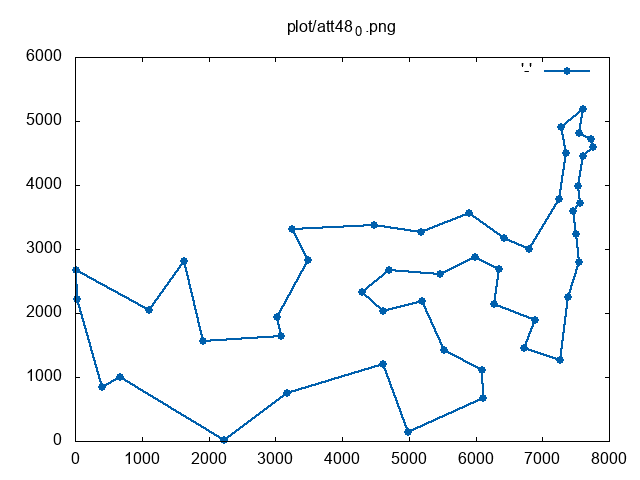
\includegraphics[width=\columnwidth]{../res/att48_0.png}
		\caption{Optimal subtour (cost $ = 10628 $, exec time = $ 0.76 $ s)}
		\label{fig:att48_best}
	\end{subfigure}
	\begin{subfigure}{.5\textwidth}
		\centering
		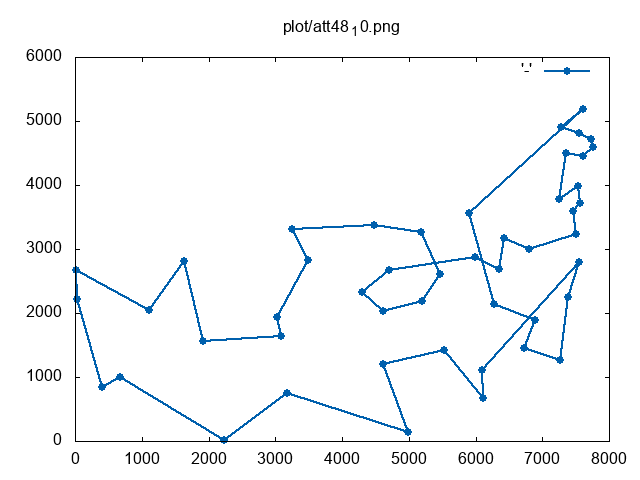
\includegraphics[width=\columnwidth]{../res/att48_10.png}
		\caption{Best Greedy (cost $ = 12012 $, exec time = $ 10^{-6} $s)}
		\label{fig:att48_GREEDY}
	\end{subfigure}
	\begin{subfigure}{.5\textwidth}
	\centering
	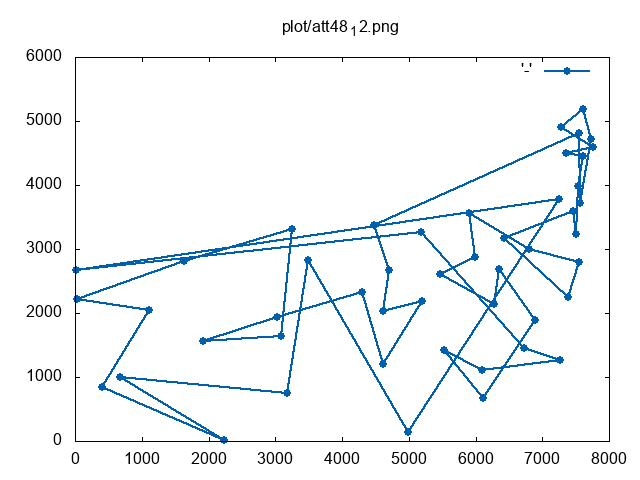
\includegraphics[width=\columnwidth]{../res/att48_12_1.png}
	\caption{GRASP (cost = 21824, exec time = $ 10^{-6} $s)}
	\label{fig:att48_GRASP1}
	\end{subfigure}
	\begin{subfigure}{.5\textwidth}
	\centering
	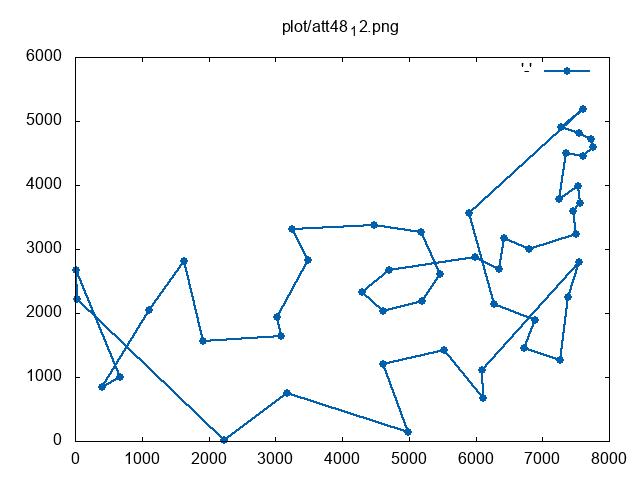
\includegraphics[width=\columnwidth]{../res/att48_12_2.png}
	\caption{GRASP (cost = 12576, exec time = $ 10^{-6} $s)}
	\label{fig:att48_GRASP2}
	\end{subfigure}
	\begin{subfigure}{.5\textwidth}
	\centering
	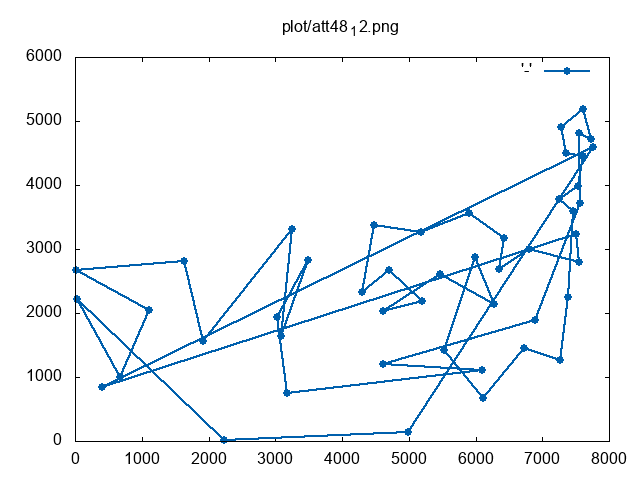
\includegraphics[width=\columnwidth]{../res/att48_12_3.png}
	\caption{GRASP (cost = 22179, exec time = $ 10^{-6} $s)}
	\label{fig:att48_GRASP3}
	\end{subfigure}
	\begin{subfigure}{.5\textwidth}
	\centering
	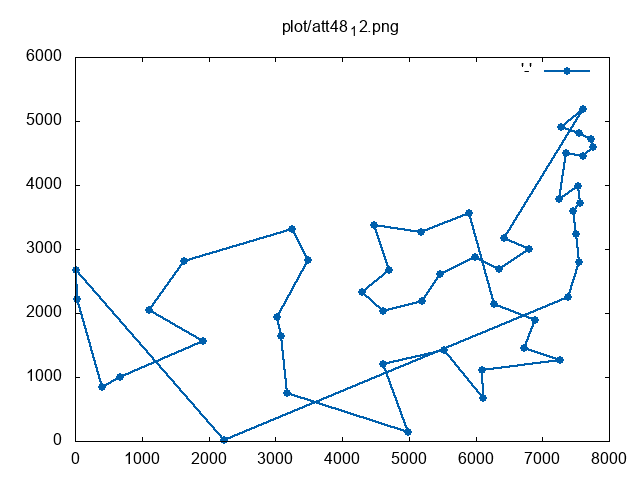
\includegraphics[width=\columnwidth]{../res/att48_12_4.png}
	\caption{GRASP (cost = 13198, exec time = $ 10^{-6} $s)}
	\label{fig:att48_GRASP4}
	\end{subfigure}
	\caption{Differences of Greedy and GRASP tour for att48.tsp instace.}
	\label{fig:att48_diff}
\end{figure}

\section{Insertion Heuristic}
